
\documentclass[12pt]{article}

\usepackage{graphicx}
\usepackage{verbatim}
\usepackage[colorlinks=true]{hyperref}
\usepackage{natbib}

\title{Enabling naturalistic, long-duration and continual animal experimentation}

\begin{document}

\maketitle

\tableofcontents
\pagebreak

\section{Vision}

For over four years, at the Sainsbury Wellcome Centre and Gatsby Computational
Neuroscience Unit, we have been developing the AEON platform, a set of hardware
and software tools that support a new type of experimentation, where animals
are allowed to express ethologically-relevant behaviors, in naturalistic
environments, and in long-duration experiments, while their behavior and
neural activity is monitored continuously for weeks to months.
%
We have used this platform to characterize foraging behavior in both solitary
and groups of mice~\citep{aeonRepo} (Figure~\ref{fig:aeonPlatform}).

Our US partner, the Allen Institute for Neural Dynamics, is using the AEON
platform in continuous learning experiments, where mice freely explore odors
continuously for days to weeks~\citep{carlsPapers}.

This is an unprecedented type of experimentation that \ldots

Several groups around the world are performing this new type of
experimentation~\cite{}.

We have built the AEON platform, and have used it to collect weeks- to
months-long NaLoDuCo experimental data. We next propose to develop advanced
machine learning methods and intelligent visualisations to extract meaning from
this data (Aim 1).

A central aim of both the SWC/GCNU and AIND is to contribute to open science.
We thus propose to create software infrastructure to openly disseminate
NaLoDuCo recordings, visualisation and data analysis methods (Aim 2).

Over more than four years we have developed the AEON platform following high
software engineering practices. It is an open source platform that anybody can
use and modify~\citep{aeonResources}. We want it to become the standard platform for the collection
of NaLoDuCo experimental data.
%
We are currently using AEON on two new NaLoDuCo experiments: (1) odor learning
experiments, lasting for days to weeks, lead by Dr.~Carl Schoonover at the
AIND, and (2) foraging experiments in very large arenas (eight meters in
diameter), lead by Prof.~Tiago Branco at the SWC.
%
We will extend and validate the functionality of the AEON platform by applying
it to these and new NaLoDuCo experiments.
%
A key functionality that we propose to add as part of this project is real-time
machine learning, to allow to control AEON experiments with live inferences
(Aim 3).

\begin{figure}
    \begin{center}
        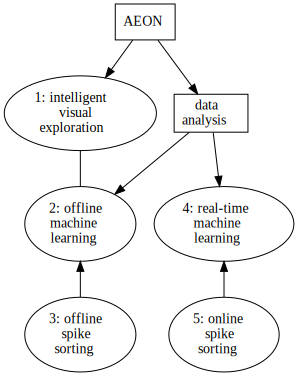
\includegraphics[width=5in]{figures/aims.png}
    \end{center}
    \caption{Proposal aims}
    \label{fig:aims}
\end{figure}

\subsection*{Aim 1: create infrastructure for open dissemination of NaLoDuCo
experimental recordings}

The dissemination of NaLoDuCo recordings is not
trivial, as datasets generated by this new type of experimentation are
enormous. For instance, the size of a dataset generated from a one week
recording of behavioral and neural activity from a foraging mouse in SWC
experiments exceeds 200 terabytes. It will take users several days to download
these datasets over standard Internet connections.

Instead of bringing data to users, we will bring users to data, by storing
datasets in the cloud (or in institutional clusters), and providing
\textbf{cloud software to allow users to visually explore and statistically
analyse behavioural and neural NaLoDuCo datasets where they live}
(Figure~\ref{fig:aims}, left box).

Our statistical analysis of neural time series will require knowledge of the
spiking activity of single units; i.e., spike sorting. In long-duration
experiments with freely moving animals spike sorting is a challenging problem,
because movements of recording probes change the shape of spike waveforms over
time and complicate the assignment of spikes to units based on their waveforms.
We will address this problem by developing \textbf{spike sorting methods for
long-duration and continual, long-duration and high-channel-count recordings}
(Figure~\ref{fig:aims}, left box).

\subsection*{Aim 2: create real-time machine learning methods for intelligent
experimentation}

In small-animal Neuroscience, most often statistical processing of neural time series is
performed offline;
i.e., experimental data is collected, saved to files, which are later
statistically processed, with no runtime constraints. Most often all
experimental data is processes at the same time; i.e., batch processing.

A new online statistical processing approach is now emerging in small-animal Neuroscience,
where data is processes while it is being collected, and at the speed of data
generation~\citep{vermaniEtAl24}.

Online methods are well suited for NaLoDuCo experimentation. In experiments
extending for weeks to months animals learn and adapt, their motivation and
fatigue may fluctuate, and experimental conditions (e.g., lighting) may change.
Offline batch processing algorithms cannot model this type of changing data.
They assume stationary data whose statistical properties do not change across
time. Differently, most online processing algorithms are robust to
these changes.
%
Also, NaLoDuCo experimentation is well suited for online methods, as the
long-duration of these experiments provide a large amount of data to accurately
fit expressive online methods.

We will \textbf{optimize methods developed for Aim~1 so that they can operate
in real time}, and focus on the following two applications of these online
methods (Figure~\ref{fig:aims}, right box).

\subsubsection*{Intelligent neuromodulation}

Brain activity can be modulated optically, chemically and
electrically~\citep{}.
%
Most commonly these modulations are done at fixed experimental times, or based on
simple behavioral or neural observations.
%
We will guide optogenetic manipulations based on inferences from advanced
machine learning methods.

For example, a scientists may hypothesize that a peak in a neural latent
variable, inferred from a prefrontal cortex population, signals the moment when
mice decide to begin a foraging bout.  To test this, she estimates latent
variables from prefrontal cortex activity online, and forecasts when this peak
will occur. She then optogenetically inactivates the neural population at the
forecasted time.  Because the inactivations prevented the mouse from initiating
a foraging bout, her hypothesis is supported.

\subsubsection*{Intelligent experimental data storage}

As the duration of NaLoDuCo experiments becomes longer, and the volume of the
behavioral and neural recordings becomes larger, it will be unfeasible to
store all raw data. We will be forced to intelligently decide, in real time,
subsets of data to discard. Real-time machine learning methods can guide the
decision of what subset of data to discard, as exemplified below.

If we are recording videos from a mouse foraging in a large arena
with ten high-resolution cameras, it would save considerable storage if at any
time we only save videos from cameras capturing the mouse at that time.  This
could be done by tracking the position of the mouse in real time with
probabilistic machine learning methods. Then, when the confidence of the
tracking is high, we would only save videos of cameras capturing the mouse at
the tracked position, but when the confidence is low, we would save all videos.

\section{Approach}

\subsubsection{Use Case}
\label{sec:useCase}

% foraging problem
%
% problems:
%   - body part tracking,
%   - kinematics inference,
%   - pose estimation,
%   - regression to test relations between the probability of entering a patch and regressors,
%   - policy inference,
%   - low-dimensional representation of neural activity,
%   - testing causality (neural manipulation)
%
% methods we could use to address the previous problems:
%

\subsection{Offline machine learning}

Extracting meaning from long-duration and continual recordings opens
challenges and opportunities that we will address and exploit in this project,
as we describe below.

\subsubsection{Challenges}

\subsubsection*{Non-stationarities}

Conventional offline methods used to characterize neural time series assume
that the statistical characteristics of the modeled data do not change with
time (i.e., that the probability of the data is time invariant --
stationarity). This assumption may be valid for shorter experiments. However,
for long-duration experiments, where animals learn and adapt, where their
motivation fluctuates, and their activity is modulated by circadian, utradiem
and peridiem rhythms, the stationarity assumption may not hold.

The field of adaptive signal processing~\citep{haykin02} develops algorithms to
characterize non-stationary systems. There is no unique solution to optimally
process any non-stationary signal. Instead, adaptations to specific algorithms
have been developed to improve their performance in non-stationary
environments.
%
For example, the recursive least-squares algorithm \citep[][Chapter
9]{haykin02} is an adaptation of the ordinary least square algorithm to perform
linear regression with non-stationary data.
%
For artificial neural networks, a very large number of strategies have been
developed to address data non-stationarity. To mention a few, continual
learning has introduced algorithms like  Elastic Weight
Consolidation~\citep[EWC][]{} and Learning Without Forgetting~\citep[LwF][]{}
to allow models to adapt to changes over time without catastrophic forgetting.
Also from this subfield is the Experience Replay (ER) algorithm that stores
past data samples in a buffer and replays them alongside new data during
training. A different type of strategy is used by ensemble methods~\citep{},
which combine multiple models trained on different time windows to capture
evolving data patterns.


\subsubsection*{Long processing times for very large datasets}

Neural and behavioral data analysis is most effective when computations can be
performed quickly, ideally in real time. Very slow computations discourage data
analysis, and hurts scientific discovery. The large dataset sizes generated by
NaLoDuCo experimentation are an important challenge for fast data analysis.

To overcome this limitation, we will leverage distributed computing, a paradigm
in which tasks and data are divided across multiple computers. Instead of
relying on a single powerful machine, distributed computing accelerates
processing by executing multiple parts of a computation in parallel.

\begin{comment}
For distributed computing to deliver substantial speed improvements,
computations must be decomposable into independent parallel tasks. While not
all algorithms naturally support such decomposition, distributed computing
remains valuable even for non-parallelizable algorithms. For instance, it
enables efficient hyperparameter optimization, where multiple algorithm
configurations can be tested in parallel, significantly reducing overall
runtime.
\end{comment}

We will develop parallel implementations of the of core machine learning
algorithms for behavioral and neural data analysis (Section~\ref{sec:coreMLAlgorithms}).
These implementations will use Apache Spark\footnote{https://spark.apache.org/}
to parallelise pre-processing and feature extraction, and
Ray\footnote{https://docs.ray.io/} to parallelise machine learning and deep
learning functionality.

\subsubsection{Opportunities}

\subsubsection{Outputs}

\subsection{Visual Exploration}

\subsection{Spike Sorting}

\subsection{Dissemination}

\subsection{Online Machine Learning}

\subsection{Software and Infrastructure}
% Python, Kubernetes, Apache Spark, Ray, Bonsai, Bonsai.ML

\end{document}
